%% Minimun Test File
%% Encoding: UTF-8
%% xelatex test.tex
%% 正确的PDF编译结果:
% 显示"中文测试"和英文内容
% 嵌入AdobeSongStd和NimbusRomNo9字体
% 英文字符正确连字(ligature)
% textsc正确工作
\documentclass[12pt,a4paper,UTF8,adobefonts]{ctexbook}
% Font Setting
\usepackage{fontspec}
\usepackage{times}
\usepackage[T1]{fontenc}
% Graph
\usepackage{graphicx}
\usepackage{subfigure}
\usepackage{ccaption}
% 设置图形文件的搜索路径
\graphicspath{{figure/}{figures/}{logo/}{logos/}{graph/}{graphs}}
% 如果插入的图片没有指定扩展名,那么依次搜索下面的扩展名所对应的文件
\DeclareGraphicsExtensions{.pdf,.eps,.png,.jpg,.jpeg}
% 重定义\nobreakspace命令
\DeclareRobustCommand\nobreakspace{\leavevmode\nobreak\ }

\begin{document}

中文测试\\
Times Fonts Here ff fi fl ffi \textsc{PostScript} % 检查连字

\begin{figure}
  \centering
  \subfigure[EPS Figure]{
    \label{fig:demo:a} %% label for first subfigure
    
\includegraphics[width=0.3\textwidth]{chap2/testeps}}
  \hspace{1in}
  \subfigure[PDF Figure]{
    \label{fig:demo:b} %% label for second subfigure
    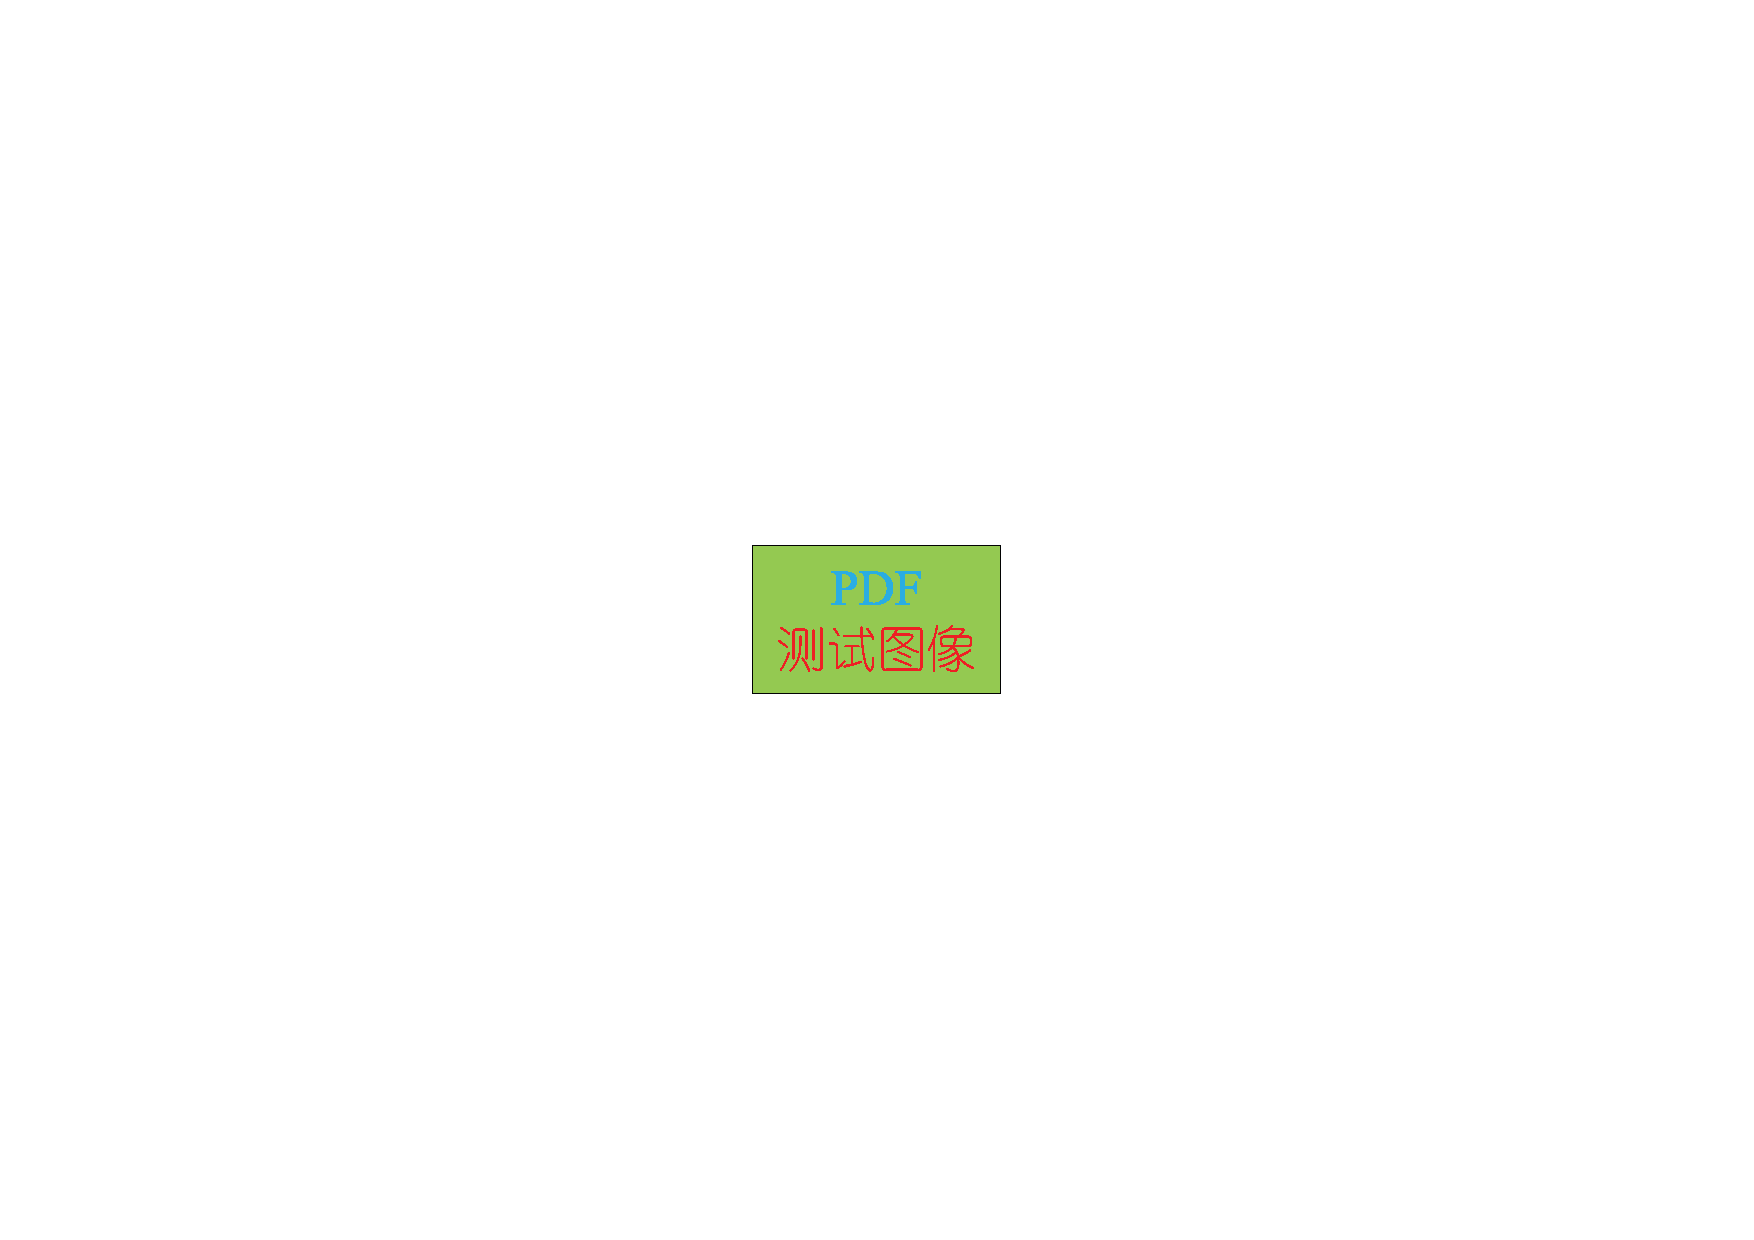
\includegraphics[angle=-90,origin=br,width=0.3\textwidth]{chap2/testpdf}}
  \\ % newline
  \subfigure[PNG Figure]{
    \label{fig:demo:c} %% label for third subfigure
    
\includegraphics[width=0.3\textwidth]{chap2/testpng}}
  \hspace{1in}
  \subfigure[JPG Figure]{
    \label{fig:demo:d} %% label for fourth subfigure
    
\includegraphics[width=0.3\textwidth]{chap2/testjpg}}
  \bicaption[fig:demo]{插入图像}{插入图像的例子}{Fig}{A demo}
\end{figure}


\end{document}
